\chapter{Statistiek van chemische metingen}\label{ch:b2:measurement-statistics}

Twee laboratoria meten het lood in hetzelfde kraanwater en rapporteren 9.6 en \qty{11.2}{\micro g/L}.
De richtwaarde voor drinkwater is \qty{10}{\micro g/L}. Is het water drinkbaar? Zijn de twee
laboratoria het eigenlijk wel oneens, of zijn beide resultaten dezelfde waarde, gezien door de spreiding van twee
metingen? Een getal uit een analyse betekent niets zonder zijn onzekerheid, en dit hoofdstuk geeft
de middelen om die te berekenen: de statistiek van herhaalde metingen, de voortplanting van onzekerheden
door een berekening, ijking met de kleinste-kwadratenmethode, en de grenzen waaronder een methode niets ziet.
% ledger: who:lead

\begin{omfigure}
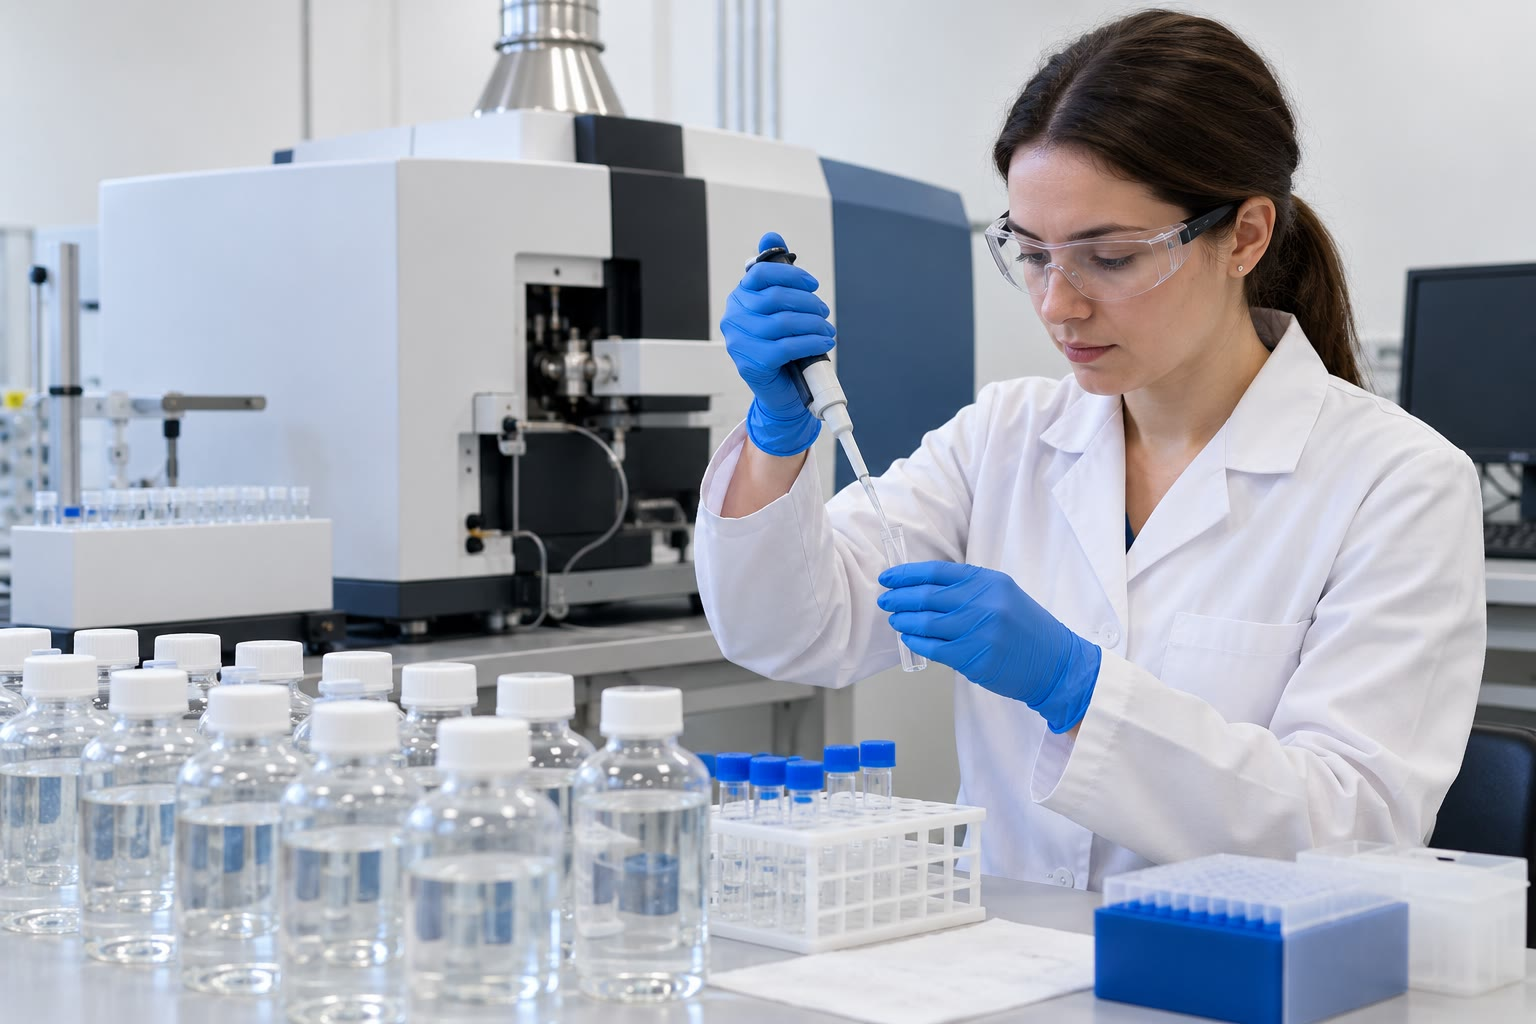
\includegraphics[width=0.56\linewidth]{images/book3/ai/b2-34-water-lab.jpg}

{\small Een laboratorium voor wateranalyse: monsterflessen, een laborant die pipetteert, een elementanalysator
op de achtergrond (illustratie).}
\end{omfigure}

\begin{recall}
Het deel van jaar~1: meetonzekerheid, standaardonzekerheid, evaluaties van type A en type B,
uitgebreide onzekerheid, relatieve onzekerheid, de genormaliseerde afwijking $z$ tussen twee waarden, en de
belofte van een bewijs van $u(\bar x) = s/\sqrt n$ en van een algemene voortplantingsregel. Het schoolboek: de
ijklijn. \Cref{ch:b2:mass-spec-atomic}: atoomabsorptie.
\end{recall}

\section{Herhaalde metingen}

Herhaal een meting en de resultaten spreiden. We behandelen elk resultaat $x_i$ als een toevalsvariabele met
gemiddelde $\mu$ (de waarde die de methode gemiddeld zou geven) en standaardafwijking $\sigma$; wanneer veel
kleine onafhankelijke oorzaken optellen, volgen de resultaten de normale (gaussische) verdeling, met ongeveer 68~\% ervan
binnen $\mu \pm \sigma$ en 95~\% binnen $\mu \pm 1.96\sigma$.

\begin{definition}[Spreiding]\label{def:b2:measurement-statistics:dispersion}
Voor $n$ resultaten $x_1, \dots, x_n$ met gemiddelde $\bar x$ is de \emph{experimentele
standaardafwijking}\index{experimentele standaardafwijking} $s = \sqrt{\sum (x_i - \bar x)^2/(n-1)}$; ze
schat $\sigma$. De \emph{standaardafwijking van het gemiddelde}\index{standaardafwijking van het gemiddelde} is
de standaardafwijking van $\bar x$ over vele reeksen van $n$ resultaten, geschat door $s/\sqrt n$.
\end{definition}

De deler $n - 1$ in plaats van $n$ corrigeert voor het feit dat de afwijkingen genomen worden ten opzichte van $\bar x$,
dat zelf uit dezelfde gegevens berekend is, waardoor ze iets te klein uitvallen: $n - 1$ is het aantal
onafhankelijke afwijkingen, de vrijheidsgraden.

\begin{theorem}[Variantie van het gemiddelde]\label{thm:b2:measurement-statistics:mean-variance}
Als $x_1, \dots, x_n$ onafhankelijk zijn, elk met variantie $\sigma^2$, dan is $\operatorname{var}(\bar x) =
\sigma^2/n$: de \omterm{def:b2:measurement-statistics:dispersion}{standaardafwijking van het gemiddelde} is $\sigma/\sqrt n$.
\end{theorem}

\begin{proof}
Voor onafhankelijke variabelen is de variantie van een som de som van de varianties, en
$\operatorname{var}(cX) = c^2\operatorname{var}(X)$. Dus $\operatorname{var}(\bar x) =
\operatorname{var}\bigl(\tfrac1n\sum x_i\bigr) = \tfrac{1}{n^2}\sum\operatorname{var}(x_i) =
\tfrac{1}{n^2}\,n\sigma^2 = \sigma^2/n$. Door $\sigma$ te vervangen door haar schatting $s$ krijg je de standaardonzekerheid van
type A, $u(\bar x) = s/\sqrt n$, die in het deel van jaar~1 aangenomen werd.
\end{proof}

\section{Betrouwbaarheidsintervallen}

\begin{definition}[Betrouwbaarheidsinterval]\label{def:b2:measurement-statistics:confidence}
Een \emph{betrouwbaarheidsinterval}\index{betrouwbaarheidsinterval} met \emph{betrouwbaarheidsniveau}\index{betrouwbaarheidsniveau}
$1 - \alpha$ (vaak 95~\%) is een interval dat uit de gegevens berekend wordt met een regel die, toegepast op
vele reeksen, de ware waarde bevat in een fractie $1 - \alpha$ ervan. Voor het gemiddelde van $n$ resultaten is het
$\bar x \pm t\,s/\sqrt n$, waarin $t$ de \emph{coëfficiënt van Student}\index{coefficient van Student@coëfficiënt van Student} is
voor $n - 1$ vrijheidsgraden en dat niveau.
\end{definition}

\begin{proposition}[Verdeling van Student]\label{prop:b2:measurement-statistics:student}
Voor $n$ onafhankelijke normaal verdeelde resultaten volgt $T = (\bar x - \mu)/(s/\sqrt n)$ de verdeling van Student met
$n - 1$ vrijheidsgraden, waarvan de dichtheid evenredig is met $(1 + t^2/\nu)^{-(\nu+1)/2}$, met
$\nu = n - 1$. Ze is breder dan de normale verdeling en nadert die naarmate $n$ groeit.
\end{proposition}

\admitted

Delen door $s$ in plaats van door de onbekende $\sigma$ voegt de spreiding van $s$ zelf toe, en die is groot wanneer $n$
klein is; vandaar de zwaardere staarten, en coëfficiënten groter dan 1.96. De tabel geeft de coëfficiënten voor 95~\%,
berekend uit de dichtheid.

\begin{omfigure}
\begin{minipage}[c]{0.56\linewidth}
\begin{tikzpicture}
\begin{axis}[width=\linewidth, height=4.8cm, xmin=-5, xmax=5, ymin=0, ymax=0.43,
  xlabel={$t$}, ylabel={dichtheid}, label style={font=\small}, tick label style={font=\scriptsize},
  legend style={font=\scriptsize, at={(0.98,0.98)}, anchor=north east}, legend cell align=left]
\addplot[omThm, thick] table[x=t, y=nu2] {figdata/out/bachelor-2-regression-c.dat};
\addplot[omMeth, thick] table[x=t, y=nu5] {figdata/out/bachelor-2-regression-c.dat};
\addplot[black, thick, dashed] table[x=t, y=normal] {figdata/out/bachelor-2-regression-c.dat};
\legend{$\nu = 2$, $\nu = 5$, normaal}
\end{axis}
\end{tikzpicture}
\end{minipage}\hfill
\begin{minipage}[c]{0.4\linewidth}\centering
\small
\begin{tabular}{rr}
\hline
$\nu = n - 1$ & $t$ (95~\%) \\
\hline
1 & 12.706 \\
2 & 4.303 \\
3 & 3.182 \\
4 & 2.776 \\
5 & 2.571 \\
9 & 2.262 \\
20 & 2.086 \\
$\infty$ & 1.960 \\
\hline
\end{tabular}
\end{minipage}
\par\vspace{4pt}

{\small Dichtheden van Student voor 2 en 5 vrijheidsgraden tegenover de normale verdeling, en de tweezijdige
coëfficiënten voor 95~\%, berekend door de dichtheid te integreren (de laatste regel is de normale verdeling).}
% figdata: bachelor-2/regression.py parts c, e
\end{omfigure}

\begin{method}[Een betrouwbaarheidsinterval voor een gemiddelde]\label{met:b2:measurement-statistics:confidence-interval}
\begin{enumerate}
  \item Bereken $\bar x$ en $s$ van de $n$ resultaten; controleer dat geen enkel resultaat grof afwijkt.
  \item Lees $t$ af voor $\nu = n - 1$ bij het gekozen niveau.
  \item Rapporteer $\bar x \pm t\,s/\sqrt n$, met de onzekerheid afgerond op één of twee beduidende cijfers
        en het gemiddelde op dezelfde decimaal.
  \item Om te vergelijken met een referentiewaarde $x_{\mathrm{ref}}$, bereken je $|\bar x - x_{\mathrm{ref}}|/(s/\sqrt
        n)$: boven $t$ is het verschil significant op dat niveau; eronder tonen de gegevens geen
        verschil (wat niet bewijst dat er geen is).
\end{enumerate}
\end{method}

\section{Voortplanting van onzekerheden}

\begin{theorem}[Wet van de voortplanting van onzekerheden]\label{thm:b2:measurement-statistics:propagation}
Als $y = f(x_1, \dots, x_n)$, waarin de $x_i$ onafhankelijk zijn met standaardonzekerheden $u(x_i)$ die klein
genoeg zijn opdat $f$ erover bijna lineair is, dan geldt
\begin{equation*}
u^2(y) = \sum_{i=1}^{n}\left(\frac{\partial f}{\partial x_i}\right)^2 u^2(x_i).
\end{equation*}
\end{theorem}

\begin{proof}
In eerste orde (Taylor) is $y - f(\mu_1, \dots, \mu_n) \approx \sum c_i(x_i - \mu_i)$ met $c_i = \partial
f/\partial x_i$ bij de gemiddelden. De variantie van een lineaire combinatie van onafhankelijke variabelen is
$\sum c_i^2\operatorname{var}(x_i)$ (zoals in \cref{thm:b2:measurement-statistics:mean-variance}); met
$\operatorname{var}(x_i) = u^2(x_i)$ is dit het resultaat.
\end{proof}

\begin{corollary}[Sommen en producten]\label{cor:b2:measurement-statistics:products}
Bij een som of verschil tellen de standaardonzekerheden kwadratisch op: $u^2(x_1 \pm x_2) = u^2(x_1) +
u^2(x_2)$. Bij een product of quotiënt $y = x_1^{a}x_2^{b}\cdots$ tellen de relatieve onzekerheden kwadratisch
op, elk gewogen met haar exponent: $\bigl(u(y)/y\bigr)^2 = a^2\bigl(u(x_1)/x_1\bigr)^2 +
b^2\bigl(u(x_2)/x_2\bigr)^2 + \cdots$
\end{corollary}

\begin{proof}
Bij een som zijn de partiële afgeleiden $\pm1$. Voor $y = x_1^ax_2^b$ is $\partial y/\partial x_1 =
a\,y/x_1$ en $\partial y/\partial x_2 = b\,y/x_2$; de stelling geeft $u^2(y) = a^2y^2u^2(x_1)/x_1^2 +
b^2y^2u^2(x_2)/x_2^2$; deel door $y^2$.
\end{proof}

\begin{method}[Voortplanten]\label{met:b2:measurement-statistics:propagate}
\begin{enumerate}
  \item Schrijf het resultaat als een formule van de gemeten grootheden; som elke ingang op met zijn
        standaardonzekerheid (type A of B).
  \item Werk bij producten en quotiënten met relatieve onzekerheden, bij sommen met absolute;
        neem anders partiële afgeleiden.
  \item Combineer kwadratisch; zoek de dominante term: de andere verbeteren is verspilde moeite.
  \item Vermenigvuldig met de dekkingsfactor (2, of de $t$ van Student wanneer de dominante term uit weinig
        herhalingen komt) voor een uitgebreide onzekerheid.
\end{enumerate}
\end{method}

\section{IJking}

\begin{definition}[IJkkromme]\label{def:b2:measurement-statistics:calibration}
Een \emph{ijkkromme}\index{ijkkromme} verbindt het signaal $y$ van een instrument met de
concentratie $x$, aan de hand van standaarden met bekende concentratie. De \emph{kleinste-kwadratenrechte}\index{kleinste-kwadratenrechte}
$y = a + bx$ is de rechte die $S = \sum (y_i - a -
bx_i)^2$ minimaliseert; elke $e_i = y_i - a - bx_i$ is een \emph{residu}\index{residu}.
\end{definition}

\begin{theorem}[Kleinste-kwadratenrechte]\label{thm:b2:measurement-statistics:least-squares}
Met $\bar x$, $\bar y$ de gemiddelden, $S_{xx} = \sum(x_i - \bar x)^2$ en $S_{xy} = \sum(x_i - \bar x)(y_i -
\bar y)$ heeft de \omterm{def:b2:measurement-statistics:calibration}{kleinste-kwadratenrechte}
\begin{equation*}
b = \frac{S_{xy}}{S_{xx}}, \qquad a = \bar y - b\bar x.
\end{equation*}
\end{theorem}

\begin{proof}
$S$ is een kwadratische functie van $a$ en $b$. Haar partiële afgeleiden worden nul in het minimum:
$\partial S/\partial a = -2\sum(y_i - a - bx_i) = 0$ geeft $a = \bar y - b\bar x$; invullen in
$\partial S/\partial b = -2\sum x_i(y_i - a - bx_i) = 0$ geeft $\sum x_i\bigl((y_i - \bar y) - b(x_i -
\bar x)\bigr) = 0$, dus $S_{xy} = bS_{xx}$ (omdat $\sum \bar x(y_i - \bar y) = \sum \bar x(x_i - \bar
x) = 0$). De tweede afgeleiden vormen de matrix
\[\begin{pmatrix} 2n & 2\sum x_i\\ 2\sum x_i & 2\sum x_i^2\end{pmatrix},\]
waarvan de diagonaal positief is en waarvan de determinant $4nS_{xx}$ positief is wanneer de $x_i$ niet allemaal
gelijk zijn: het stationaire punt is een minimum.
\end{proof}

\begin{proposition}[Een concentratie aflezen]\label{prop:b2:measurement-statistics:interpolation}
Voor $n$ standaarden met residuele standaardafwijking $s_{y/x} = \sqrt{\sum e_i^2/(n-2)}$ heeft een monster dat
$m$ keer gemeten is met gemiddeld signaal $\bar y_0$ de waarde $x_0 = (\bar y_0 - a)/b$ en de standaardafwijking
\begin{equation*}
s_{x_0} = \frac{s_{y/x}}{b}\sqrt{\frac1m + \frac1n + \frac{(\bar y_0 - \bar y)^2}{b^2S_{xx}}},
\end{equation*}
te gebruiken met de $t$ van Student voor $n - 2$ vrijheidsgraden.
\end{proposition}

\admitted

De drie termen onder de wortel zijn de spreiding van de metingen van het monster, de onzekerheid op de hoogte
van de rechte en die op haar helling; de laatste verdwijnt in het midden van het ijkbereik, en daar
worden monsters dus het best afgelezen.

\begin{omfigure}
\begin{tikzpicture}
\begin{axis}[width=0.5\linewidth, height=5cm, xmin=-1, xmax=22, ymin=0, ymax=0.22,
  xlabel={lood (\unit{\micro g/L})}, ylabel={absorbantie}, label style={font=\small},
  tick label style={font=\scriptsize}, scaled y ticks=false,
  yticklabel style={/pgf/number format/fixed, /pgf/number format/precision=2}]
\addplot[omDef, thick] table[x=x, y=line] {figdata/out/bachelor-2-regression-b.dat};
\addplot[only marks, mark=*, mark size=1.8pt, omThm] table[x=x, y=A] {figdata/out/bachelor-2-regression-a.dat};
\end{axis}
\end{tikzpicture}\hfill
\begin{tikzpicture}
\begin{axis}[width=0.5\linewidth, height=5cm, xmin=-1, xmax=22, ymin=-0.002, ymax=0.002,
  xlabel={lood (\unit{\micro g/L})}, ylabel={residu}, label style={font=\small},
  tick label style={font=\scriptsize}, scaled y ticks=false, ycomb,
  yticklabel style={/pgf/number format/fixed, /pgf/number format/precision=3},
  extra y ticks={0}, extra y tick style={grid=major, grid style={black!50}}]
\addplot[omThm, thick, mark=*, mark size=1.6pt] table[x=x, y=res] {figdata/out/bachelor-2-regression-a.dat};
\end{axis}
\end{tikzpicture}

{\small IJking van lood door atoomabsorptie met grafietoven bij \qty{283.3}{nm} (gegevens voor de oefening,
gebruikt in het probleem). Links: de vijf standaarden en de \omterm{def:b2:measurement-statistics:calibration}{kleinste-kwadratenrechte}. Rechts: de \omterm{def:b2:measurement-statistics:calibration}{residuen}, klein
en zonder patroon: een rechte volstaat.}
% figdata: bachelor-2/regression.py parts a, b
% ledger: asd:Pb283
\end{omfigure}

\begin{method}[IJken]\label{met:b2:measurement-statistics:calibrate}
\begin{enumerate}
  \item Maak vijf of meer standaarden die het verwachte bereik overspannen, in dezelfde matrix als de monsters,
        en een blanco.
  \item Pas de \omterm{def:b2:measurement-statistics:calibration}{kleinste-kwadratenrechte} aan; zet de \omterm{def:b2:measurement-statistics:calibration}{residuen} uit. Een gebogen patroon betekent dat de respons niet
        lineair is: versmal het bereik of pas een kromme aan. Eén groot \omterm{def:b2:measurement-statistics:calibration}{residu} wijst op een foute standaard.
  \item Lees de monsters af, bij voorkeur rond het midden van het bereik, in meervoud; bereken $x_0$ en
        $s_{x_0}$.
  \item Rapporteer $x_0 \pm t\,s_{x_0}$ na correctie voor elke verdunning, met de voortgeplante onzekerheid
        van de verdunning erbij als die niet verwaarloosbaar is.
\end{enumerate}
\end{method}

\begin{definition}[Standaardadditie]\label{def:b2:measurement-statistics:standard-addition}
Bij de \emph{standaardadditiemethode}\index{standaardadditiemethode} worden bekende hoeveelheden analyt
toegevoegd aan gelijke porties van het monster zelf; het signaal wordt uitgezet tegen de toegevoegde concentratie,
en de concentratie van de analyt in het monster is de afstand van de oorsprong tot het punt waar
de rechte, geëxtrapoleerd naar signaal nul, de as snijdt, $a/b$.
\end{definition}

\begin{method}[Standaardadditie]\label{met:b2:measurement-statistics:standard-addition}
\begin{enumerate}
  \item Gebruik ze wanneer de matrix van het monster de respons verandert (zouten, zuren, organisch materiaal), zodat
        standaarden in zuiver water een verkeerde helling zouden geven.
  \item Voeg aan gelijke porties stijgende bekende hoeveelheden toe, verdun alles tot hetzelfde volume, meet.
  \item Pas de rechte aan; de concentratie in de gemeten oplossingen is $a/b$; corrigeer voor de verdunning.
  \item De respons moet lineair zijn vanaf nul: controleer de \omterm{def:b2:measurement-statistics:calibration}{residuen}.
\end{enumerate}
\end{method}

\begin{omfigure}
\begin{tikzpicture}
\begin{axis}[width=0.62\linewidth, height=5cm, xmin=-4, xmax=7, ymin=0, ymax=0.42,
  xlabel={toegevoegde concentratie (\unit{mg/L})}, ylabel={absorbantie}, label style={font=\small},
  tick label style={font=\scriptsize}, axis lines=left, scaled y ticks=false,
  yticklabel style={/pgf/number format/fixed, /pgf/number format/precision=1}]
\draw[black!40] (axis cs:0,0) -- (axis cs:0,0.42);
\addplot[omDef, thick, densely dashed] table[x=x, y=line] {figdata/out/bachelor-2-regression-d-line.dat};
\addplot[only marks, mark=*, mark size=1.8pt, omThm] table[x=x, y=A] {figdata/out/bachelor-2-regression-d.dat};
\draw[<->, omMeth, thick] (axis cs:-3.11,0.06) -- (axis cs:0,0.06); \node[omMeth, below, font=\scriptsize] at (axis cs:-0.8,0.055) {$a/b$};
\end{axis}
\end{tikzpicture}

{\small Standaardadditie (gegevens voor de oefening): absorbantie van een monster waaraan 0, 2, 4 en
\qty{6}{mg/L} analyt toegevoegd is. De rechte bereikt signaal nul bij \qty{-3.11}{mg/L}: de gemeten oplossing
bevatte \qty{3.11}{mg/L}.}
% figdata: bachelor-2/regression.py part d
\end{omfigure}

\section{Detectie, kwantificering en validatie}

\begin{definition}[Grenzen]\label{def:b2:measurement-statistics:limits}
De \emph{detectiegrens}\index{detectiegrens} van een methode is de kleinste concentratie waarvan het
signaal onderscheiden kan worden van dat van een blanco met een vastgelegd klein risico op een valse detectie; de
\emph{kwantificeringsgrens}\index{kwantificeringsgrens} is de kleinste concentratie die
gemeten kan worden met een aanvaardbare relatieve onzekerheid.
\end{definition}

\begin{proposition}[Gangbare schattingen]\label{prop:b2:measurement-statistics:lod}
Met $s_{\mathrm{blank}}$ de standaardafwijking van herhaalde blancosignalen en $b$ de helling van de
ijklijn geldt $x_{\mathrm{LOD}} \approx 3s_{\mathrm{blank}}/b$ en $x_{\mathrm{LOQ}} \approx
10s_{\mathrm{blank}}/b$.
\end{proposition}

\begin{proof}[Redenering]
Als blancosignalen normaal verdeeld zijn met standaardafwijking $s_{\mathrm{blank}}$, overschrijdt een blanco zijn gemiddelde met
meer dan $3s_{\mathrm{blank}}$ met een kans van ongeveer 0.13~\% (eenzijdige staart van de normale verdeling voorbij
3 standaardafwijkingen): wie een signaal boven die drempel ``gedetecteerd'' noemt, verwart zelden een blanco met
een monster. Een signaal $10s_{\mathrm{blank}}$ boven de blanco heeft een relatieve standaardafwijking van ongeveer
10~\%, de gebruikelijke drempel voor een kwantitatief resultaat. Delen door $b$ zet signalen om in
concentraties.
\end{proof}

\begin{definition}[Validatie]\label{def:b2:measurement-statistics:validation}
\emph{Juistheid}\index{juistheid} is de mate waarin het gemiddelde van een groot aantal resultaten de ware
waarde benadert; hun verschil is de \emph{bias}\index{bias}. \emph{Precisie}\index{precisie} is de mate waarin
onafhankelijke resultaten met elkaar overeenkomen, uitgedrukt als standaardafwijking:
\emph{herhaalbaarheid}\index{herhaalbaarheid} onder dezelfde omstandigheden (zelfde operator, instrument,
laboratorium, korte tijd), \emph{reproduceerbaarheid}\index{reproduceerbaarheid} onder gewijzigde omstandigheden
(verschillende laboratoria). \emph{Methodevalidatie}\index{methodevalidatie} is de set experimenten
die voor een methode de juistheid, de precisie, de lineariteit en het bereik, en de detectie- en
\omterm{def:b2:measurement-statistics:limits}{kwantificeringsgrens} vastleggen.
\end{definition}

De \omterm{def:b2:measurement-statistics:validation}{juistheid} wordt gecontroleerd met een gecertificeerd referentiemateriaal of door toevoegingen; de \omterm{def:b2:measurement-statistics:validation}{precisie} met herhalingen in
één laboratorium en met vergelijkingen tussen laboratoria. Een methode kan precies maar vertekend zijn: elk
resultaat dicht bij de andere en allemaal fout. \omterm{def:b2:measurement-statistics:validation}{Precisie} is geen bewijs van \omterm{def:b2:measurement-statistics:validation}{juistheid}.

\begin{history}[Student, 1908]
\begin{minipage}[t]{0.17\linewidth}
\vspace{0pt}
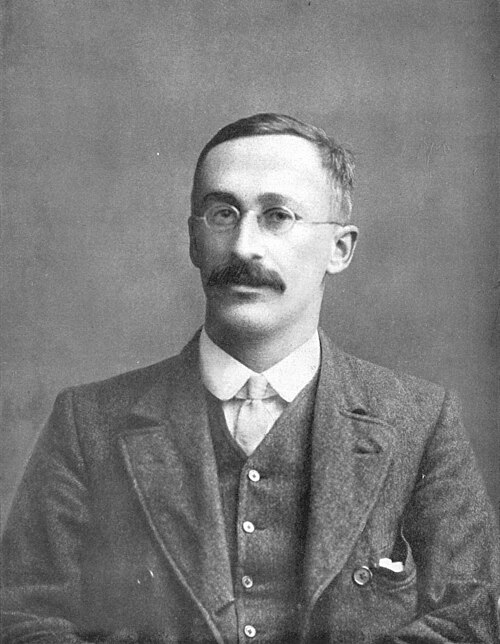
\includegraphics[width=\linewidth]{images/book3/gosset.jpg}
\end{minipage}\hfill
\begin{minipage}[t]{0.79\linewidth}
\vspace{0pt}
William Sealy Gosset, een chemicus die voor een brouwerij werkte, moest grondstoffen beoordelen op basis van zeer weinig monsters,
veel te weinig voor de normale verdeling. In 1908 publiceerde hij de verdeling van het gemiddelde gedeeld door de standaardafwijking
van de steekproef, onder het pseudoniem ``Student'', omdat zijn werkgever het personeel niet toestond onder eigen naam
te publiceren. De verdeling van Student wordt gebruikt telkens wanneer een analist een interval opgeeft uit drie of vier
herhalingen. (Foto, 1908: publiek domein; Wikimedia Commons.)
\end{minipage}
\end{history}

\section{Oefeningen}

\begin{exercise}[$\star$]\label{exo:b2:measurement-statistics:1}
Vijf titraties geven 12.45, 12.50, 12.48, 12.52 en \qty{12.46}{mL}. Bereken het gemiddelde, de
\omterm{def:b2:measurement-statistics:dispersion}{experimentele standaardafwijking} en de \omterm{def:b2:measurement-statistics:dispersion}{standaardafwijking van het gemiddelde}.
\end{exercise}

\begin{exercise}[$\star$]\label{exo:b2:measurement-statistics:2}
Geef het \omterm{def:b2:measurement-statistics:confidence}{betrouwbaarheidsinterval} bij 95~\% van het gemiddelde van oefening~1.
\end{exercise}

\begin{exercise}[$\star$]\label{exo:b2:measurement-statistics:3}
Een oplossing wordt gemaakt door $m = \qty{0.5000}{g}$ ($u = \qty{0.0002}{g}$) van een vaste stof op te lossen in een maatkolf van
$V = \qty{250.0}{mL}$ ($u = \qty{0.15}{mL}$). Bereken de relatieve standaardonzekerheid van $c = m/(MV)$,
waarbij de molaire massa nauwkeurig genoeg bekend is.
\end{exercise}

\begin{exercise}[$\star$]\label{exo:b2:measurement-statistics:4}
Pas de \omterm{def:b2:measurement-statistics:calibration}{kleinste-kwadratenrechte} aan door $(0, 0.02)$, $(1, 0.21)$, $(2, 0.39)$, $(3, 0.62)$.
\end{exercise}

\begin{exercise}[$\star\star$]\label{exo:b2:measurement-statistics:5}
Een gecertificeerde referentieoplossing bevat \qty{10.00}{mg/L} van een element. Vijf analyses geven een gemiddelde van
\qty{10.12}{mg/L} met $s = \qty{0.08}{mg/L}$. Is de methode vertekend op het niveau van 95~\%?
\end{exercise}

\begin{exercise}[$\star\star$]\label{exo:b2:measurement-statistics:6}
Een concentratie hydroniumionen is bekend met een relatieve standaardonzekerheid van 2~\%. Wat is de
standaardonzekerheid van de pH?
\end{exercise}

\begin{exercise}[$\star\star$]\label{exo:b2:measurement-statistics:7}
Tien blanco's hebben $s = 0.0012$ absorbantie-eenheden; de helling van de ijklijn is \qty{0.0098}{L/\micro g}.
Schat de \omterm{def:b2:measurement-statistics:limits}{detectiegrens} en de \omterm{def:b2:measurement-statistics:limits}{kwantificeringsgrens}.
\end{exercise}

\begin{exercise}[$\star\star$]\label{exo:b2:measurement-statistics:8}
In het standaardadditie-experiment van de figuur waren de vier porties gemaakt door
\qty{10.0}{mL} monster te verdunnen tot \qty{50.0}{mL}. Geef de concentratie in het monster.
\end{exercise}

\begin{exercise}[$\star\star$]\label{exo:b2:measurement-statistics:9}
In een interlaboratoriumstudie haalt elk laboratorium $s = \qty{0.05}{mg/L}$ op zijn eigen herhalingen, maar
de resultaten van verschillende laboratoria spreiden met $s = \qty{0.15}{mg/L}$. Geef de naam van de twee grootheden en
leg het verschil uit.
\end{exercise}

\begin{exercise}[$\star\star\star$]\label{exo:b2:measurement-statistics:10}
Toon aan dat de \omterm{def:b2:measurement-statistics:calibration}{kleinste-kwadratenrechte} door $(\bar x, \bar y)$ gaat en dat de som van haar \omterm{def:b2:measurement-statistics:calibration}{residuen} nul is.
\end{exercise}

\begin{exercise}[$\star\star\star$]\label{exo:b2:measurement-statistics:11}
Een stockoplossing wordt honderdmaal verdund, ofwel in één stap (\qty{1.000}{mL} in \qty{100.0}{mL}), ofwel
in twee stappen van tienmaal (\qty{10.00}{mL} in \qty{100.0}{mL}, twee keer). Standaardonzekerheden: pipet van 1 mL
\qty{0.006}{mL}, pipet van 10 mL \qty{0.02}{mL}, maatkolf van 100 mL \qty{0.08}{mL} (gegevens voor de oefening).
Welke route is preciezer?
\end{exercise}

\begin{exercise}[$\star\star\star$]\label{exo:b2:measurement-statistics:12}
De twee laboratoria uit de inleiding rapporteren 9.6 en \qty{11.2}{\micro g/L} met standaardonzekerheden
0.4 en \qty{0.5}{\micro g/L} (gegevens voor de oefening). Zijn hun resultaten verenigbaar? Wat zegt elk ervan over de
richtwaarde?
\end{exercise}

\section{Probleem: lood in kraanwater}

\begin{problem}[{Weekendprobleem --- een ijking voor atoomabsorptie met de kleinste-kwadratenmethode, de
concentratie van een monster met haar betrouwbaarheidsinterval, de verdunning en de grenzen, en een oordeel
tegenover de richtwaarde}]
\label{pb:b2:measurement-statistics:1}
Gegevens voor de oefening. Lood wordt gemeten door atoomabsorptie met grafietoven bij \qty{283.3}{nm}. Standaarden
(\unit{\micro g/L}; absorbantie): 0.0; 0.003, 5.0; 0.051, 10.0; 0.101, 15.0; 0.148, 20.0; 0.199. Het
kraanwater (\qty{50.0}{mL}) wordt aangezuurd met \qty{0.50}{mL} salpeterzuur; drie metingen van deze
oplossing geven 0.104, 0.098 en 0.101. Tien blanco's: 0.002, 0.004, 0.003, 0.001, 0.003, 0.005, 0.002,
0.003, 0.004, 0.003. Standaardonzekerheden van de volumes: \qty{0.03}{mL} voor 50.0 mL,
\qty{0.005}{mL} voor 0.50 mL. Richtwaarde: \qty{10}{\micro g/L}.
% ledger: who:lead, asd:Pb283

\medskip
\noindent\textbf{Deel I --- IJking.}
\begin{enumerate}
  \item Waarom worden de standaarden in hetzelfde salpeterzuur bereid als de monsters?
  \item Bereken de helling en het intercept van de \omterm{def:b2:measurement-statistics:calibration}{kleinste-kwadratenrechte}.
  \item Bereken de vijf \omterm{def:b2:measurement-statistics:calibration}{residuen}.
  \item Tonen de \omterm{def:b2:measurement-statistics:calibration}{residuen} een patroon? Besluit over de lineariteit.
  \item Bereken $s_{y/x}$.
  \item Waarom is het intercept niet nul?
  \item Wat meet de helling?
\end{enumerate}

\medskip
\noindent\textbf{Deel II --- Het monster.}
\begin{enumerate}[resume]
  \item Bereken het gemiddelde en de standaardafwijking van de drie metingen.
  \item Bereken de loodconcentratie van de gemeten oplossing.
  \item Bereken $s_{x_0}$.
  \item Hoeveel vrijheidsgraden, en welke \omterm{def:b2:measurement-statistics:confidence}{coëfficiënt van Student}?
  \item Geef het interval bij 95~\% van de concentratie in de gemeten oplossing.
  \item Waarom meet je het monster drie keer en niet één keer?
\end{enumerate}

\medskip
\noindent\textbf{Deel III --- Verdunning en grenzen.}
\begin{enumerate}[resume]
  \item Bereken de verdunningsfactor en de concentratie in het kraanwater.
  \item Plant de onzekerheid van de twee volumes voort in de verdunningsfactor.
  \item Is die onzekerheid significant naast die van de ijking?
  \item Bereken de standaardafwijking van de blanco's en de \omterm{def:b2:measurement-statistics:limits}{detectiegrens}.
  \item Bereken de \omterm{def:b2:measurement-statistics:limits}{kwantificeringsgrens}.
  \item Ligt het monster boven de \omterm{def:b2:measurement-statistics:limits}{kwantificeringsgrens}?
\end{enumerate}

\medskip
\noindent\textbf{Deel IV --- Oordeel.}
\begin{enumerate}[resume]
  \item Bevat het interval de richtwaarde?
  \item Wat zou één enkele meting van 0.104 gesuggereerd hebben?
  \item Wat betekent ``95~\% betrouwbaarheid'' hier?
  \item Hoe zou het laboratorium met meer zekerheid kunnen beslissen?
  \item Hoe zou het controleren dat de methode niet vertekend is?
  \item De richtwaarde is voorlopig ``op basis van de prestaties van de behandeling en de analytische
        haalbaarheid''. Wat betekent de tweede reden, in het licht van dit probleem?
  \item Geef de loodconcentratie van het kraanwater met haar interval bij 95~\%, en vergelijk ze met
        \qty{10}{\micro g/L}.
\end{enumerate}
\end{problem}
